\chapter{RE-008 --- Rendering Performance Findings}\label{record-156}

\noindent{\footnotesize\color{BookMuted}\path{docs/design/RE-008-perf-findings.md}\par}\smallskip

\emph{Results from the \texttt{e\allowbreak{}x\allowbreak{}a\allowbreak{}m\allowbreak{}p\allowbreak{}l\allowbreak{}e\allowbreak{}s\allowbreak{}/\allowbreak{}p\allowbreak{}e\allowbreak{}r\allowbreak{}f\allowbreak{}-\allowbreak{}g\allowbreak{}r\allowbreak{}a\allowbreak{}d\allowbreak{}i\allowbreak{}e\allowbreak{}n\allowbreak{}t} stress test, April 2026. These findings motivate \href{https://github.com/flyingrobots/bijou/blob/cbd70612140e7a450d764b3c7be1c6af878b99bc/docs/method/graveyard/legacy-backlog/asap/RE-008-byte-packed-surface-representation.md}{RE-008 --- Byte-Packed Surface Representation}.}

\section{Test setup}\label{record-156-test-setup}

\begin{itemize}
\tightlist
\item
  Terminal: iTerm2, 191×48 (9,168 cells)
\item
  Runtime: Node.js v25.8.1, tsx
\item
  Hardware: Apple Silicon Mac
\item
  Modes tested: cosine gradient (unique fg+bg per cell), ASCII perspective horizon (varying chars, few color changes), OpenSimplex noise density (varying chars, single bg), quad (all three combined)
\end{itemize}

\section{Raw numbers}\label{record-156-raw-numbers}

\begin{center}
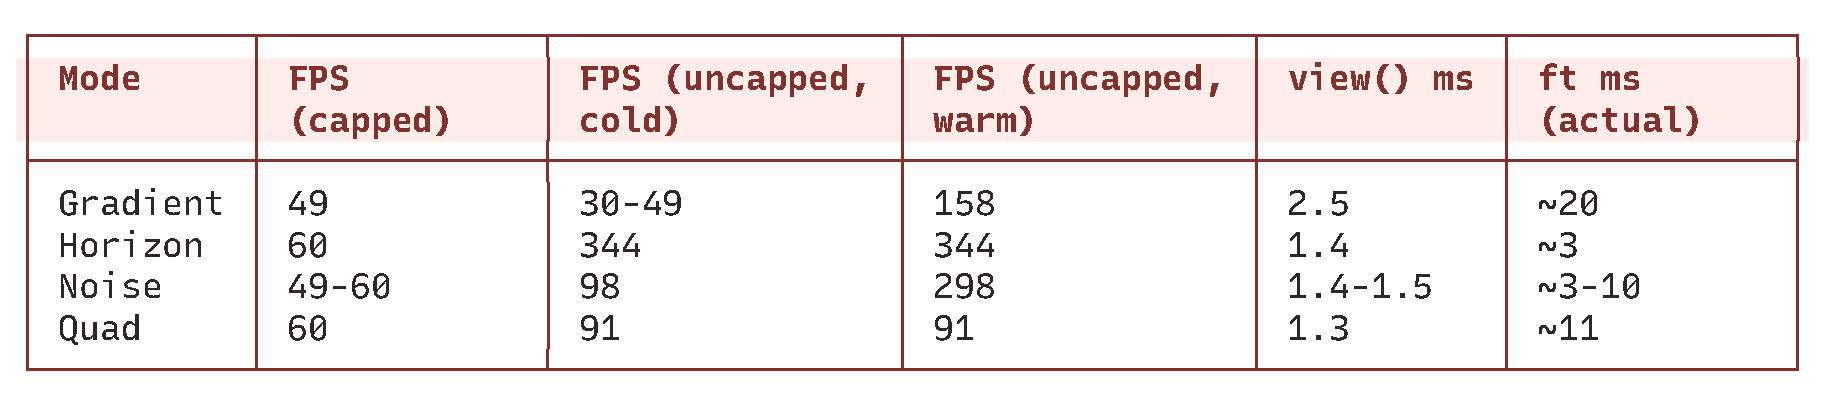
\includegraphics[width=\linewidth]{figures/tables/table-039-g1-1.pdf}
\par\smallskip{\scriptsize\color{BookMuted}Rows 1–4. Actual Bijou table component.}
\end{center}


``Warm'' means after 60+ seconds of sustained rendering, when V8 has JIT-compiled the hot paths and GC has settled.

\section{Where frame time goes}\label{record-156-where-frame-time-goes}

At 191×48 with the gradient (worst case), a frame takes \textasciitilde20ms total:

\begin{center}
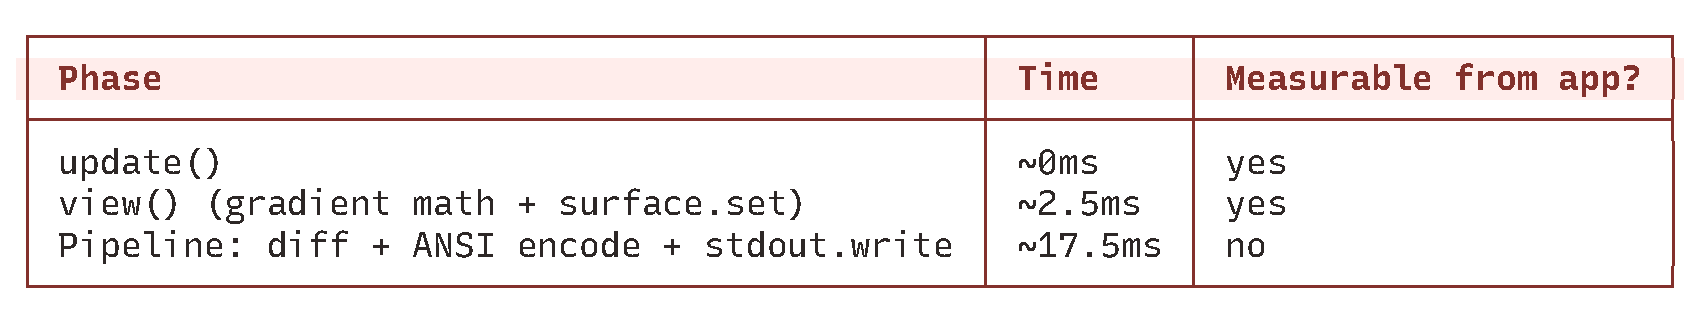
\includegraphics[width=\linewidth]{figures/tables/table-040-g1-1.pdf}
\par\smallskip{\scriptsize\color{BookMuted}Rows 1–3. Actual Bijou table component.}
\end{center}


\textbf{92\% of frame time is spent in bijou's render pipeline, not in the app's view function.} The pipeline is not observable from the app side --- there are no hooks to measure diff, paint, or output phases individually.

\section{The differ is the bottleneck}\label{record-156-the-differ-is-the-bottleneck}

The differ (\texttt{p\allowbreak{}a\allowbreak{}c\allowbreak{}k\allowbreak{}a\allowbreak{}g\allowbreak{}e\allowbreak{}s\allowbreak{}/\allowbreak{}b\allowbreak{}i\allowbreak{}j\allowbreak{}o\allowbreak{}u\allowbreak{}/\allowbreak{}s\allowbreak{}r\allowbreak{}c\allowbreak{}/\allowbreak{}c\allowbreak{}o\allowbreak{}r\allowbreak{}e\allowbreak{}/\allowbreak{}r\allowbreak{}e\allowbreak{}n\allowbreak{}d\allowbreak{}e\allowbreak{}r\allowbreak{}/\allowbreak{}d\allowbreak{}i\allowbreak{}f\allowbreak{}f\allowbreak{}e\allowbreak{}r\allowbreak{}.\allowbreak{}t\allowbreak{}s}) compares every cell in the target surface against the current surface. For cells that changed, it emits ANSI escape sequences.

The differ's performance depends on \textbf{how many unique styles appear in sequence}:

\begin{itemize}
\tightlist
\item
  \textbf{Horizon (344fps uncapped)}: most cells on a row share the same fg/bg, so the differ batches long runs of same-styled characters into single ANSI writes. Very few color change escape sequences per frame.
\item
  \textbf{Noise (298fps uncapped)}: every cell has a unique fg but all share \texttt{b\allowbreak{}g\allowbreak{}:\allowbreak{} \allowbreak{}'\allowbreak{}\#\allowbreak{}0\allowbreak{}0\allowbreak{}0\allowbreak{}0\allowbreak{}0\allowbreak{}0\allowbreak{}'}. The differ still emits per-cell fg changes but saves half the escape sequences (no bg changes).
\item
  \textbf{Gradient (158fps uncapped)}: every cell has a unique fg AND bg. The differ emits \textasciitilde9,168 color change escape sequences per frame --- one per cell. No batching is possible.
\end{itemize}

The differ also compares cells by \textbf{string equality} on \texttt{f\allowbreak{}g} and \texttt{b\allowbreak{}g} hex strings (\texttt{t\allowbreak{}a\allowbreak{}r\allowbreak{}g\allowbreak{}e\allowbreak{}t\allowbreak{}C\allowbreak{}e\allowbreak{}l\allowbreak{}l\allowbreak{}.\allowbreak{}f\allowbreak{}g\allowbreak{} \allowbreak{}=\allowbreak{}=\allowbreak{}=\allowbreak{} \allowbreak{}c\allowbreak{}u\allowbreak{}r\allowbreak{}r\allowbreak{}e\allowbreak{}n\allowbreak{}t\allowbreak{}C\allowbreak{}e\allowbreak{}l\allowbreak{}l\allowbreak{}.\allowbreak{}f\allowbreak{}g}), which is correct but slower than numeric comparison would be.

\section{Allocation pressure and GC}\label{record-156-allocation-pressure-and-gc}

Each \texttt{s\allowbreak{}u\allowbreak{}r\allowbreak{}f\allowbreak{}a\allowbreak{}c\allowbreak{}e\allowbreak{}.\allowbreak{}s\allowbreak{}e\allowbreak{}t\allowbreak{}(\allowbreak{})} call in the gradient mode produces 2 hex color strings (\texttt{r\allowbreak{}g\allowbreak{}b\allowbreak{}H\allowbreak{}e\allowbreak{}x\allowbreak{}(\allowbreak{}r\allowbreak{},\allowbreak{} \allowbreak{}g\allowbreak{},\allowbreak{} \allowbreak{}b\allowbreak{})} for fg and bg). At 9,168 cells per frame, that is \textbf{18,336 string allocations per frame}.

With surface reuse (the cached surface is not reallocated per frame), the Cell objects themselves are mutated in place via \texttt{a\allowbreak{}p\allowbreak{}p\allowbreak{}l\allowbreak{}y\allowbreak{}M\allowbreak{}a\allowbreak{}s\allowbreak{}k\allowbreak{}I\allowbreak{}n\allowbreak{}P\allowbreak{}l\allowbreak{}a\allowbreak{}c\allowbreak{}e}. But the hex color strings are always freshly allocated because they encode the current frame's computed RGB values.

\subsection{GC behavior at different modes}\label{record-156-gc-behavior-at-different-modes}

\begin{center}
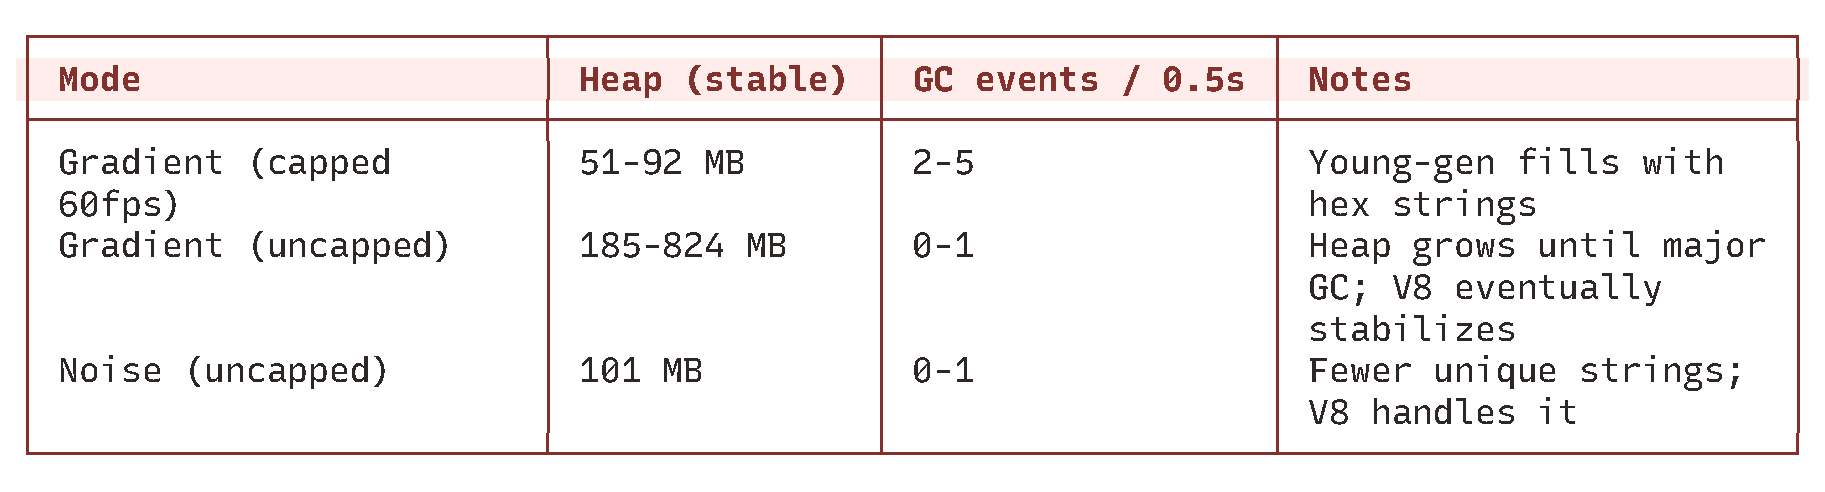
\includegraphics[width=\linewidth]{figures/tables/table-041-g1-1.pdf}
\par\smallskip{\scriptsize\color{BookMuted}Rows 1–3. Actual Bijou table component.}
\end{center}


\subsection{JIT warmup}\label{record-156-jit-warmup}

The gradient mode shows a clear warmup curve:

\begin{itemize}
\tightlist
\item
  \textbf{0-30 seconds}: 30-49fps. V8 is interpreting; GC is aggressive.
\item
  \textbf{30-60 seconds}: 80-120fps. JIT compilation kicks in.
\item
  \textbf{60+ seconds}: 150-160fps. Hot paths fully optimized, GC settled.
\end{itemize}

The noise and horizon modes warm up faster because they produce fewer unique string values per frame.

\section{What RE-008 would fix}\label{record-156-what-re-008-would-fix}

A byte-packed surface representation would eliminate:

\begin{enumerate}
\def\labelenumi{\arabic{enumi}.}
\tightlist
\item
  \textbf{18K string allocations per frame} --- colors stored as 3 bytes (R, G, B), not heap-allocated hex strings.
\item
  \textbf{String comparison in the differ} --- numeric comparison of bytes instead of \texttt{=\allowbreak{}=\allowbreak{}=} on strings.
\item
  \textbf{Hex parsing in the ANSI encoder} --- the \texttt{s\allowbreak{}t\allowbreak{}y\allowbreak{}l\allowbreak{}e\allowbreak{}.\allowbreak{}s\allowbreak{}t\allowbreak{}y\allowbreak{}l\allowbreak{}e\allowbreak{}d\allowbreak{}(\allowbreak{})} call currently parses \texttt{\#\allowbreak{}r\allowbreak{}r\allowbreak{}g\allowbreak{}g\allowbreak{}b\allowbreak{}b} back to numeric RGB to emit \texttt{\textbackslash{}\allowbreak{}x\allowbreak{}1\allowbreak{}b\allowbreak{}[\allowbreak{}3\allowbreak{}8\allowbreak{};\allowbreak{}2\allowbreak{};\allowbreak{}R\allowbreak{};\allowbreak{}G\allowbreak{};\allowbreak{}B\allowbreak{}m}. With byte-packed cells, the encoder reads bytes directly.
\item
  \textbf{The JIT warmup penalty} --- no string-heavy hot paths for V8 to deoptimize and recompile.
\end{enumerate}

\section{What DX-006 would provide}\label{record-156-what-dx-006-would-provide}

A first-class \texttt{d\allowbreak{}e\allowbreak{}b\allowbreak{}u\allowbreak{}g\allowbreak{}O\allowbreak{}v\allowbreak{}e\allowbreak{}r\allowbreak{}l\allowbreak{}a\allowbreak{}y\allowbreak{}(\allowbreak{})} component would let any bijou-tui app see these metrics without rebuilding the stats overlay from scratch. The perf gradient demo proves the concept; DX-006 extracts it into a reusable component.

\section{Pipeline observability gap}\label{record-156-pipeline-observability-gap}

The render pipeline (the illustrated sequence below) is not observable from the app side. \texttt{c\allowbreak{}o\allowbreak{}n\allowbreak{}f\allowbreak{}i\allowbreak{}g\allowbreak{}u\allowbreak{}r\allowbreak{}e\allowbreak{}P\allowbreak{}i\allowbreak{}p\allowbreak{}e\allowbreak{}l\allowbreak{}i\allowbreak{}n\allowbreak{}e} can add middleware but only appends after the default stages --- it cannot wrap them for timing. A future improvement would expose per-stage timing hooks so the debug overlay can show the full breakdown.

% Presentation of original arrow notation. See flow-manifest.json.
\begin{center}
\begin{tikzpicture}[book flow node/.style={draw=BookHeading,line width=.65pt,fill=BookPanel,rounded corners=1.5pt,align=center,inner sep=5pt,minimum height=10mm,font=\fontsize{9}{11}\selectfont,execute at begin node={\hyphenpenalty=10000\exhyphenpenalty=10000}},book flow edge/.style={-{Latex[length=2mm]},draw=BookHeading,line width=.7pt}]
\node[book flow node,text width=96mm] (n0) at (0,0.0) {Layout};
\node[book flow node,text width=96mm] (n1) at (0,-1.55) {Paint};
\node[book flow node,text width=96mm] (n2) at (0,-3.1) {Post\allowbreak{}Process};
\node[book flow node,text width=96mm] (n3) at (0,-4.65) {Diff};
\node[book flow node,text width=96mm] (n4) at (0,-6.2) {Output};
\draw[book flow edge] (n0) -- (n1);
\draw[book flow edge] (n1) -- (n2);
\draw[book flow edge] (n2) -- (n3);
\draw[book flow edge] (n3) -- (n4);
\end{tikzpicture}
\end{center}


\section{Reproducing}\label{record-156-reproducing}

\begin{CodeBlock}
npx tsx examples/perf-gradient/main.ts
\end{CodeBlock}

Keys: \texttt{1\allowbreak{}-\allowbreak{}4} switch modes, \texttt{s\allowbreak{}p\allowbreak{}a\allowbreak{}c\allowbreak{}e} toggles 60fps cap, hold mouse to reverse, \texttt{q} to quit. The stats overlay shows FPS, frame time, view time, heap/RSS/GC, and a braille line chart of view() cost.

